\documentclass{article}
\usepackage{url}
\usepackage{amsmath}
\usepackage{graphicx}

\graphicspath{ {img/} }


\title{Optimal Control}
\author{Joshua Saunders}
\date{January 2018}
\begin{document}

\maketitle

\section{State Space Review}

The state space representation of a linear time-invariant system has the 
following form:

\begin{align}     
    \dot{X}(t) &= A(t) \, X(t) \, + \, B(t) \, U(t) \label{eq:state_diff_eq}\\
    Y(t) &= C(t) \, X(t) \, + \, D(t) \, U(t) \label{eq:state_output}
\end{align}.

Equations \ref{eq:state_diff_eq} and \ref{eq:state_output} are referred to as
the \textbf{state differential equation} and \textbf{state output equation},
respectively.

\subsection{Example: Mass-Spring-Damper}

A classic example of a linear system is the Mass-Spring-Damper (MSD) system, as
shown in Figure \ref{fig:mass_spring_damper}. The differential equation for the
MSD is

\begin{equation}
    \ddot{y}(t) \, = \, -\frac{k}{m} y(t) - \frac{b}{m} \dot{y}(t) + \frac{1}{m}r(t) 
\end{equation}
\label{eq:mass_spring_damper}

\begin{figure}[h]
    \begin{center}
        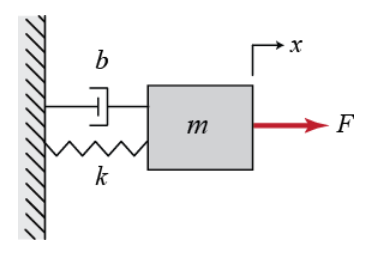
\includegraphics[scale=0.4]{mass_spring_damper}
        \caption{Linear mass-spring-damper system}
        \label{fig:mass_spring_damper}
    \end{center}
\end{figure}

By examination of Equation \ref{eq:mass_spring_damper}, we can see that the 
system has two states (the number of states is equal to the order, $n$, of the
differential equation, which in this case is $2$). We'll call these states 
$x_1$ and $x_2$ and define them in the following way:

\begin{align}
          x_1 &= y \nonumber \\
    \label{eq:x1_state} 
    \dot{x_1} &= \dot{y} = x_2 \\
          x_2 &= \dot{y} = \dot{x_1} \nonumber \\  
    \label{eq:x2_state}
    \dot{x_2} &= \ddot{y} = -\frac{k}{m} x_1 - \frac{b}{m} + \frac{1}{m} u(t)
\end{align}

\noindent where $u(t) = r(t)$. The states, $x_1$ and $x_2$, are defined by 
Equations \ref{eq:x1_state} and \ref{eq:x2_state} which respectively give the 
position and velocity of the mass, $m$.

\bibliography{bib}
\bibliographystyle{ieeetr}

\end{document}
